\indent Greedy Forwardingで局所最大問題が発生した場合に, 
Perimeter Forwardingが使用される. 
\textbf{Perimeter Forwarding}とは, 図\ref{fig:perimeter}に
示すように, 送信ノードSを中心にして宛先ノードの方向から,  
反時計回りにノードを探索し, 最初に発見したノードを
ネクストホップとして選択する方式である.

\begin{figure}
  \centering
  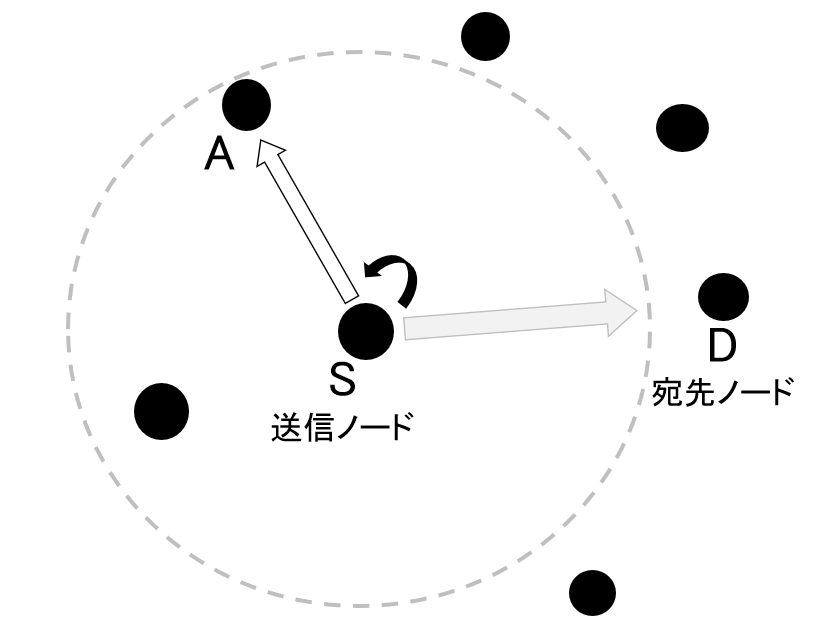
\includegraphics[scale=0.55]{figures/perimeter.png}
  \caption{Perimeter Forwarding\cite{shinato}}
  \label{fig:perimeter}
\end{figure}